\documentclass{article}
\usepackage{design}

\begin{document}

\maketitle
\newpage

\section{Introduction}
\input{build/executive_summary_md}

\input{build/ethics_statement_md}

\newpage

\tableofcontents
\newpage

\section{Background}

\subsection{Need}
\input{build/need_statement_md}

\subsection{Goal}
\input{build/goal_statement_md}

\subsection{Existing Designs}
\input{build/existing_designs_md}

\subsection{Personas}
The following are a few target audiences for our productivity device:
\input{build/camillia_md}
\input{build/elijah_md}
\input{build/linda_md}
\input{build/mary_md}
\input{build/peyton_md}

\subsection{Sustainability Statement}
\input{build/sustainability_statement_md}

\newpage

\section{Design}

\input{build/entry_design_md} % Explains the entry management concept of the device
\input{build/device_statemachine_md}

\input{build/hardware_design_md}

%device UI
\input{build/device_ui_requirements_md}
\subsubsection{User Tutorial}
In order to ensure the user fully understands how to utilize the device, a user tutorial should be provided in a similar fashion to shown in Fig. \ref{fig:user_tutorial}. Additional panels for user configuration settings should also be included for user clarity.
\begin{figure}[h]
    \begin{subfigure}{0.5\textwidth}
        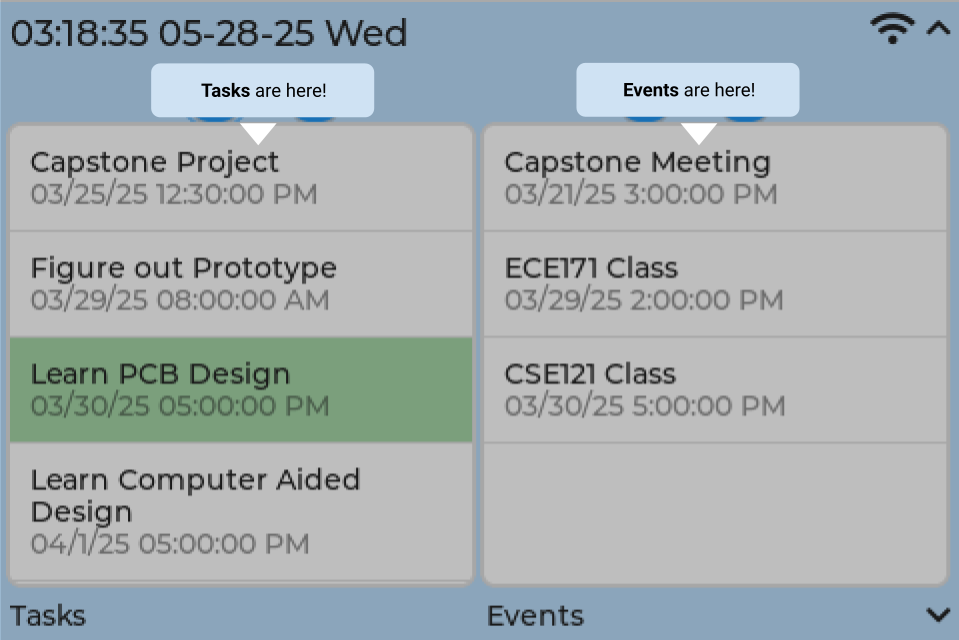
\includegraphics[width = \textwidth]{task_event.png}
        \caption{Shows what the different columns mean}
    \end{subfigure}
    \begin{subfigure}{0.5\textwidth}
        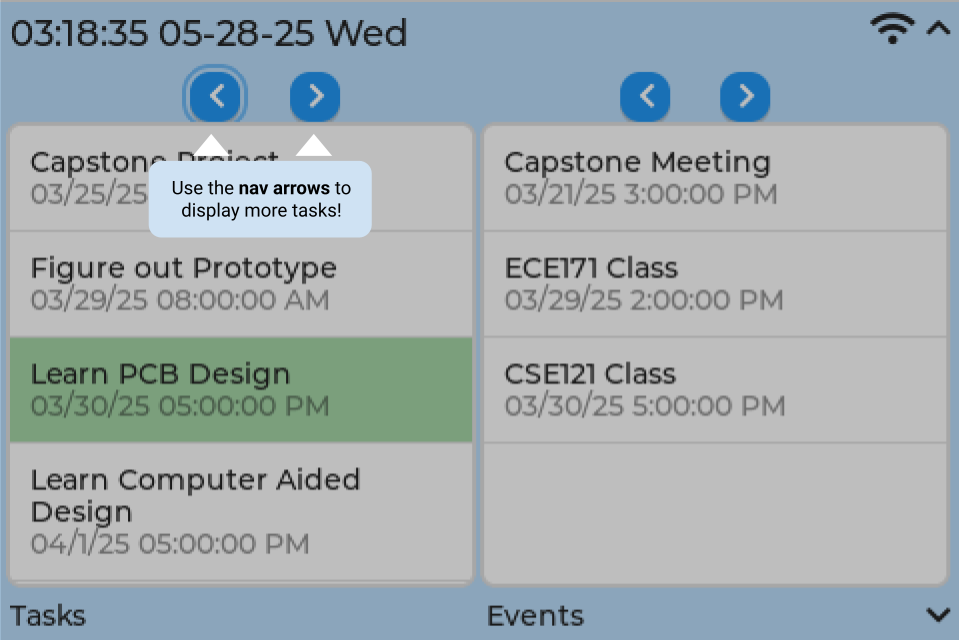
\includegraphics[width = \textwidth]{nav_arrows.png}
        \caption{Introduces navigation arrows}
    \end{subfigure}
    \begin{subfigure}{0.5\textwidth}
        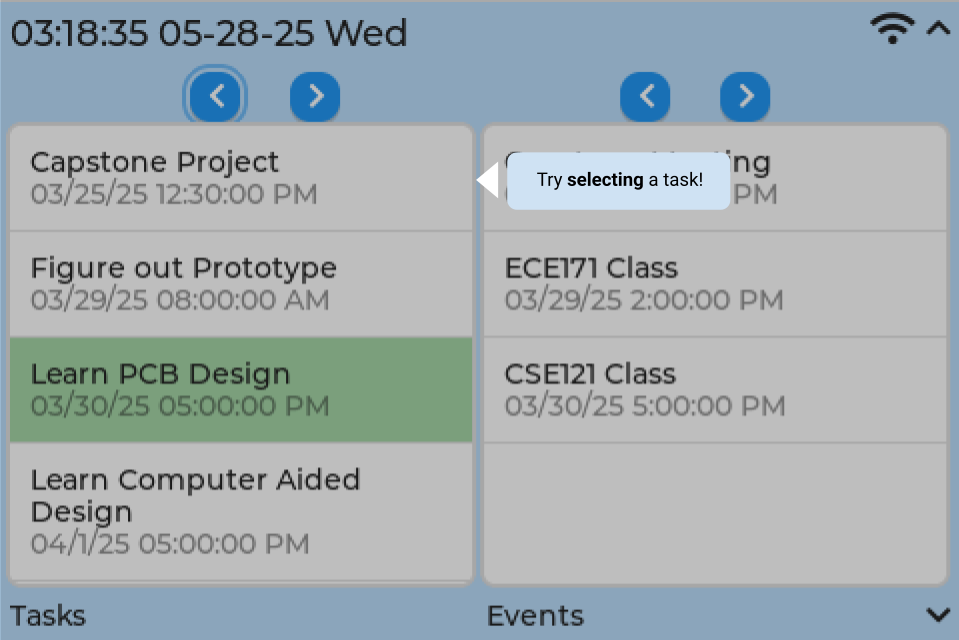
\includegraphics[width = \textwidth]{task_select.png}
        \caption{Tells user to select a task}
    \end{subfigure}
    \begin{subfigure}{0.5\textwidth}
        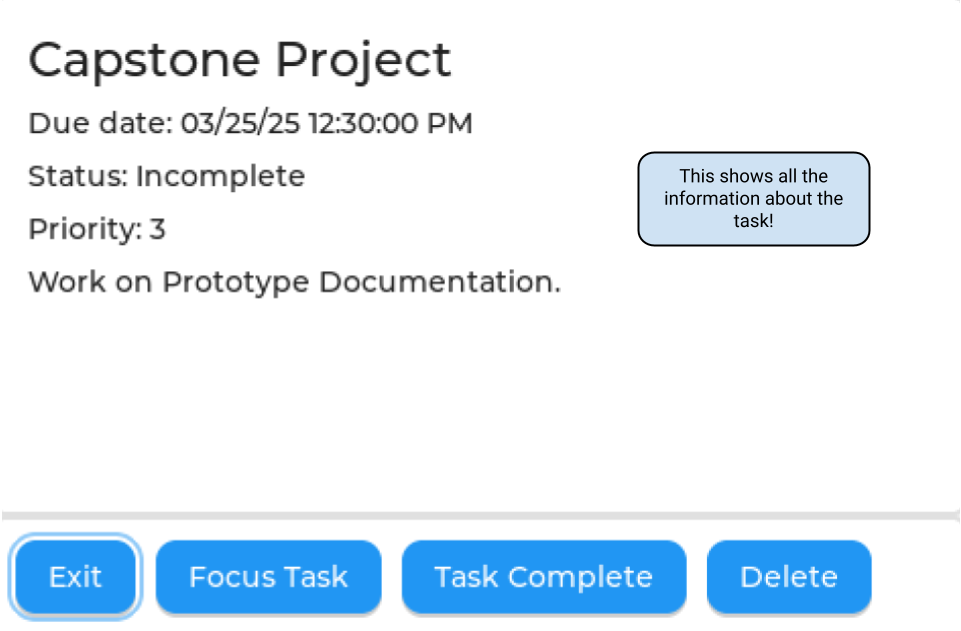
\includegraphics[width = \textwidth]{task_detail.png}
        \caption{Introduces task detail view}
    \end{subfigure}

    \begin{subfigure}{0.5\textwidth}
        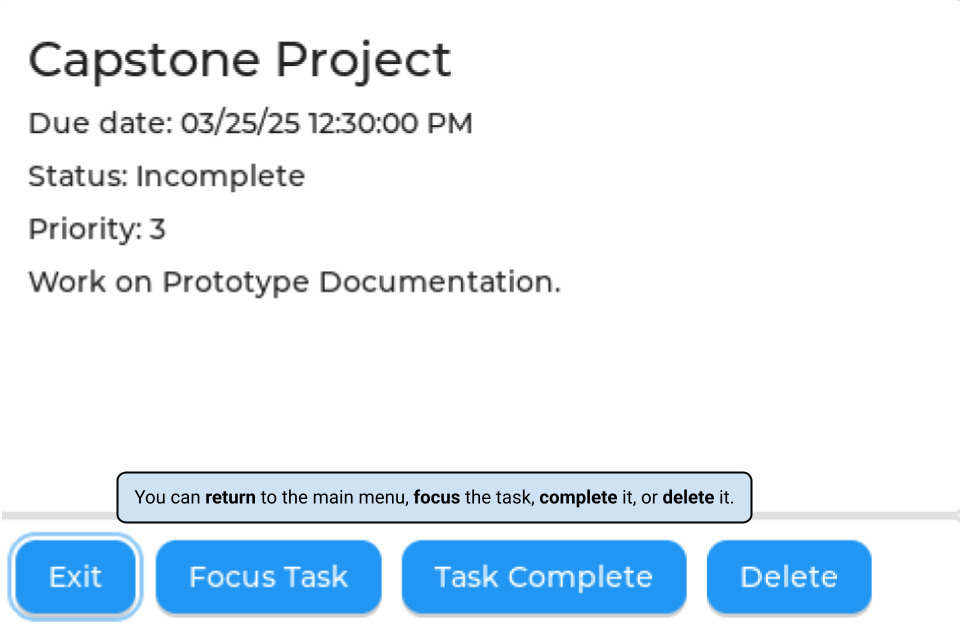
\includegraphics[width = \textwidth]{task_buttons.png}
        \caption{Introduces task interaction buttons}
    \end{subfigure}
    \begin{subfigure}{0.5\textwidth}
        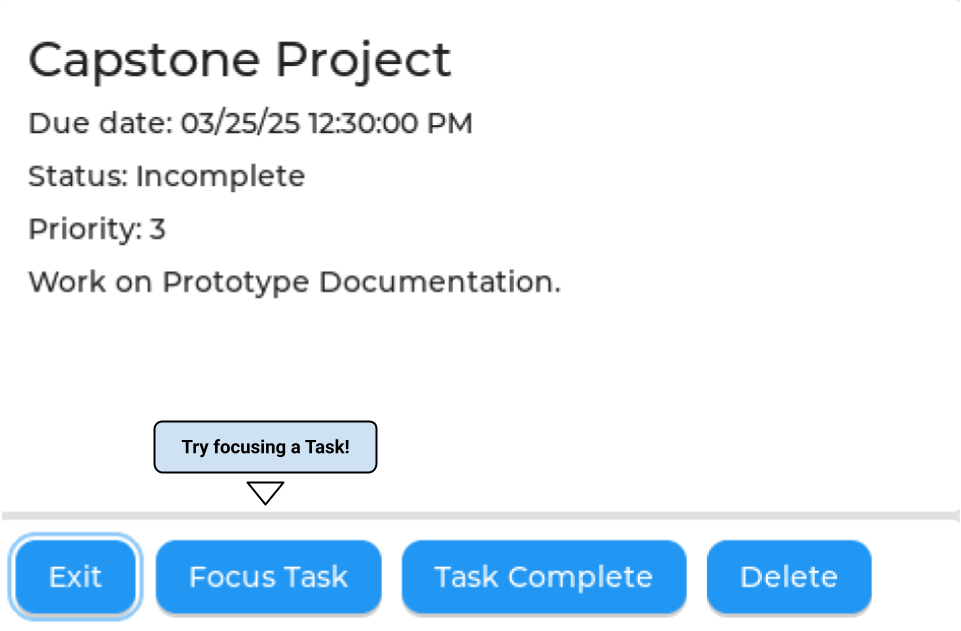
\includegraphics[width = \textwidth]{try_focus.png}
        \caption{Tells user to try focusing a task}
    \end{subfigure}
\end{figure}
\begin{figure}
    \ContinuedFloat
    \begin{subfigure}{0.5\textwidth}
        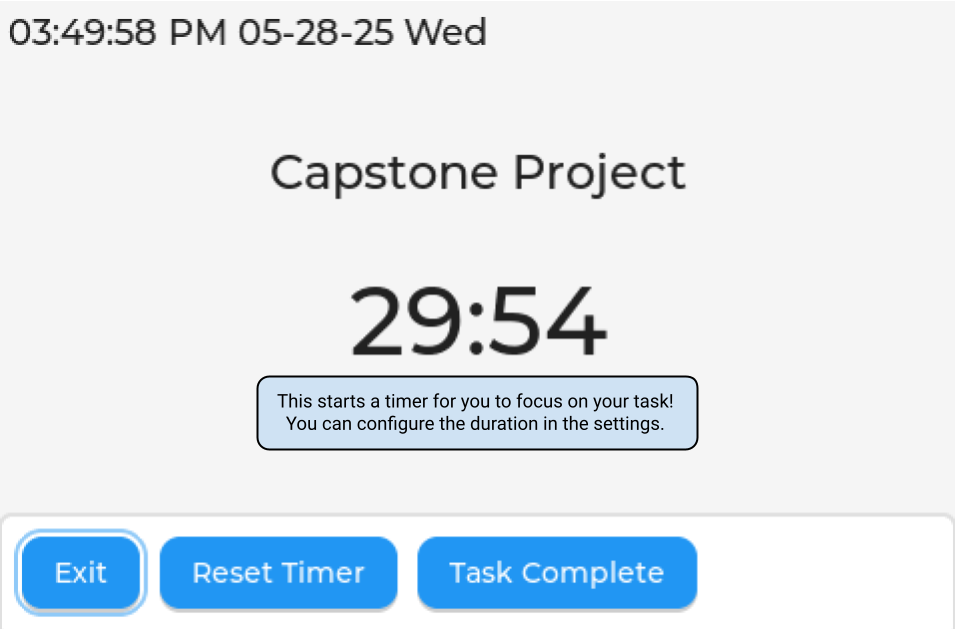
\includegraphics[width = \textwidth]{focus_tutorial.png}
        \caption{Introduces focus mode}
    \end{subfigure}
    \begin{subfigure}{0.5\textwidth}
        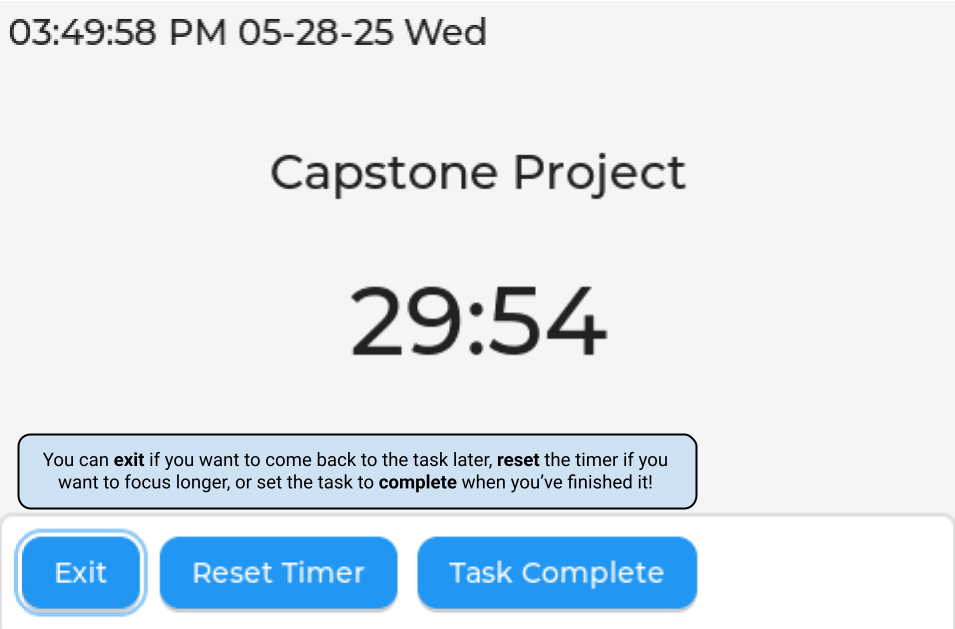
\includegraphics[width = \textwidth]{focus_buttons.png}
        \caption{Introduces focus interaction buttons}
    \end{subfigure}
    \begin{subfigure}{0.5\textwidth}
        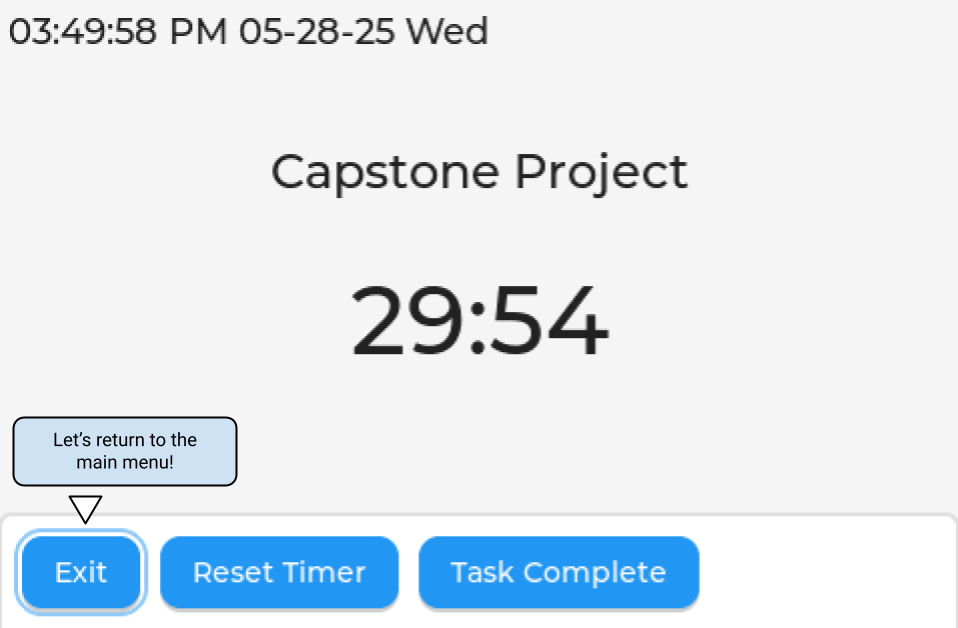
\includegraphics[width = \textwidth]{Return.png}
        \caption{Tells user to return to main menu}
    \end{subfigure}
    \begin{subfigure}{0.5\textwidth}
        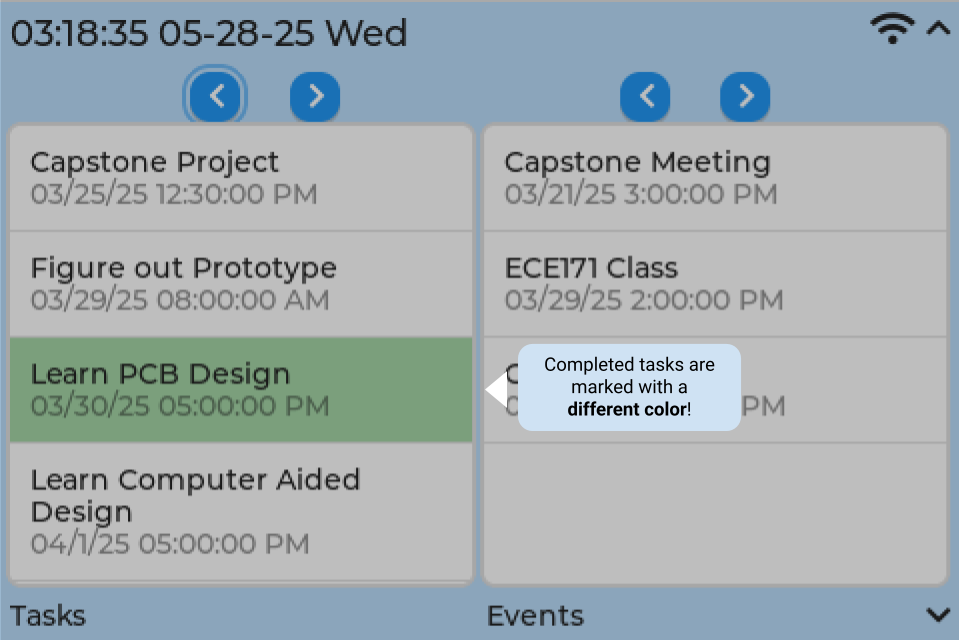
\includegraphics[width = \textwidth]{completed_task.png}
        \caption{Introduces completed tasks}
    \end{subfigure}
    \begin{subfigure}{0.5\textwidth}
        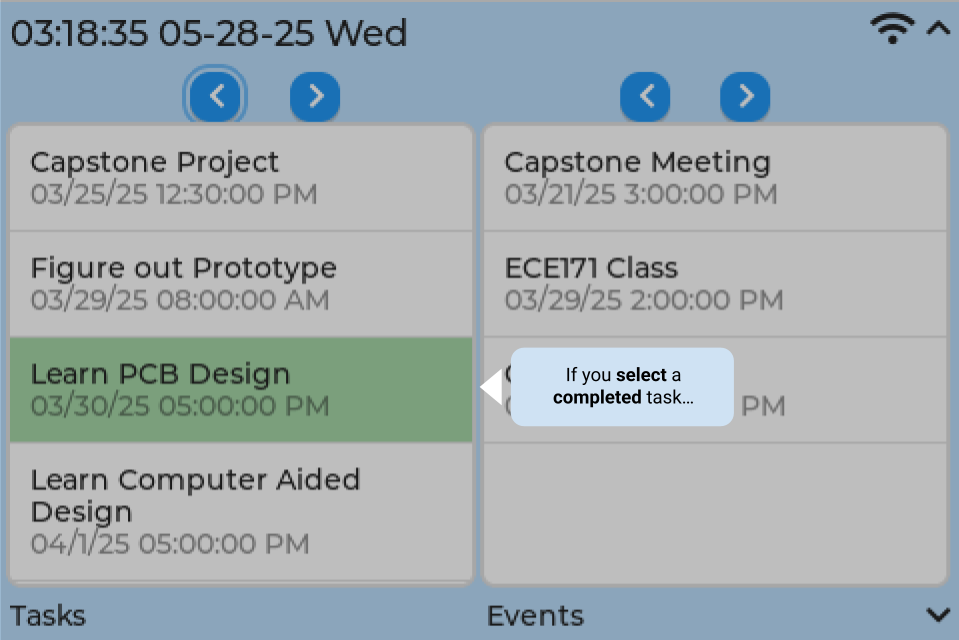
\includegraphics[width = \textwidth]{select_completed.png}
        \caption{Tells user to select completed task}
    \end{subfigure}
    \begin{subfigure}{0.5\textwidth}
        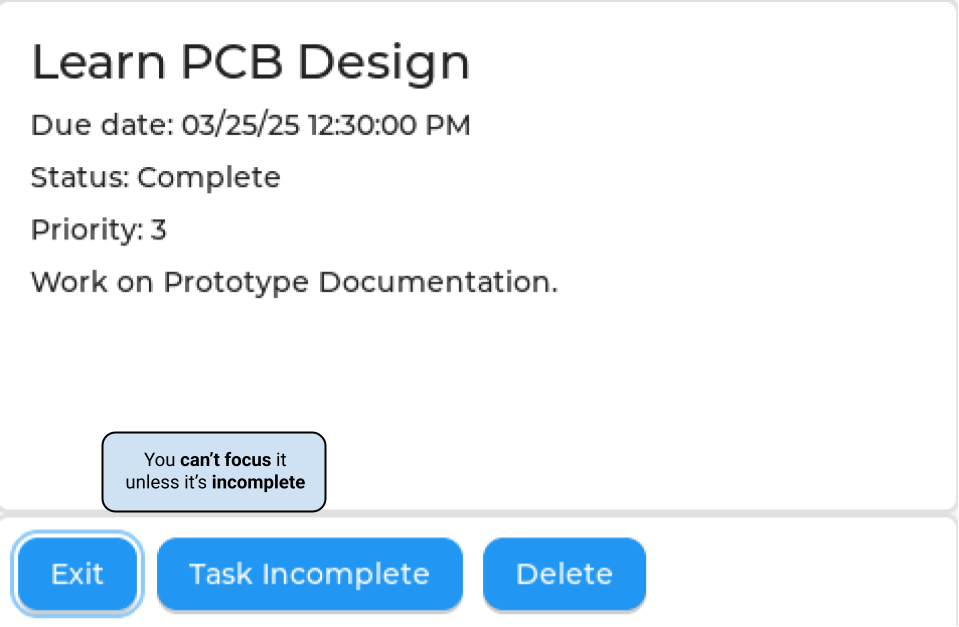
\includegraphics[width = \textwidth]{cant_focus.png}
        \caption{Informs user they cannot focus completed tasks}
    \end{subfigure}
    \end{figure}
\begin{figure}[h]
	\ContinuedFloat
    \begin{subfigure}{0.5\textwidth}
        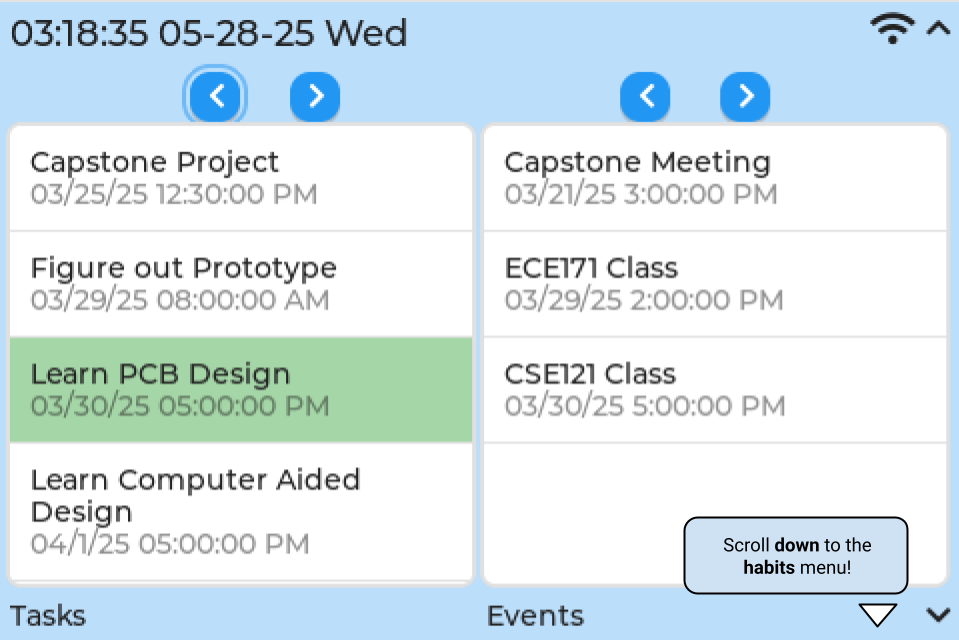
\includegraphics[width = \textwidth]{scroll_habits.png}
        \caption{Instructs user to scroll to find habits menu}
    \end{subfigure}
    \begin{subfigure}{0.5\textwidth}
        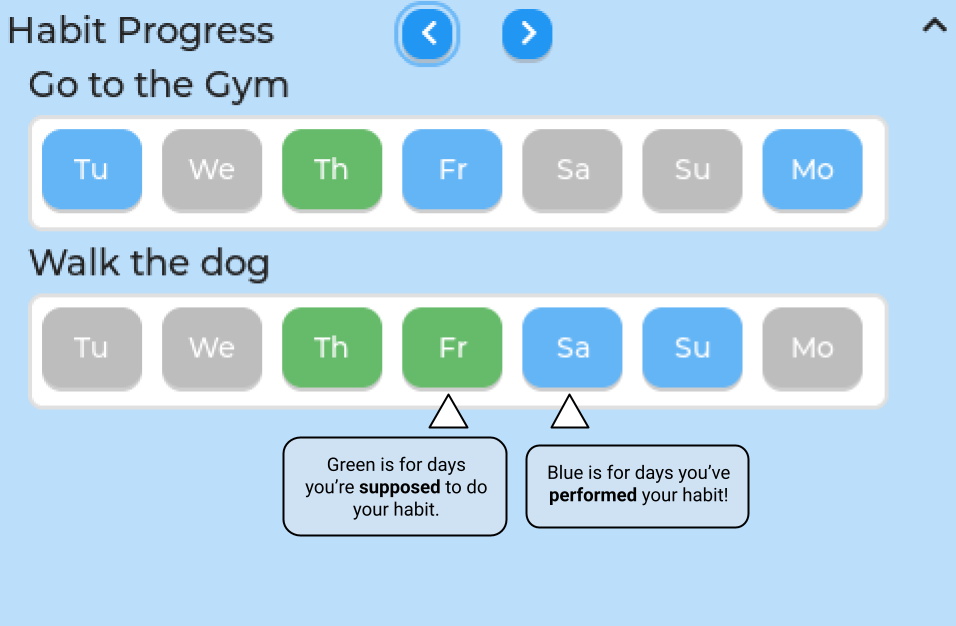
\includegraphics[width = \textwidth]{habit_tutorial.png}
        \caption{Introduces color meanings for habits}
    \end{subfigure}
\caption{User tutorial example}
\label{fig:user_tutorial}
\end{figure}

\input{build/configurable_settings_md}

\input{build/server_communication_md}

\input{build/server_design_md}

% webapp
\input{build/webapp_design_spec_md}

%phone app
\input{build/phone_app_design_md}

% Third party integration
\input{build/third-party_integration_md}

\input{build/manufactured_design_md}

\subsection{Additional Requirements}
Each device will be shipped with a unique serial number (ID) and an 8-digit code for device identification.
Alongside the device, a printed start up manual must be included with the device. An example is shown below:

\input{build/startManual_md}
Additional specifications for the manufactured design are described in section \ref{improvements} and section \ref{final_specs}.
\newpage

\subsection{Design for Manufacture and Assembly} \label{DMA}
\input{build/design_for_manufacture_and_assembly_md}
\subsection{Life Cycle Assessment}
\input{build/lifecycle_assessment_md}

\newpage

\section{Evaluation} \label{eval}

\subsection{Prototype}
\input{build/prototype_hardware_md}
\input{build/prototype_software_md}
\input{build/prototype_server_md}

\subsection{Manufactured Design Improvements} \label{improvements}
\input{build/eval_hardware_md}

\newpage

\subsection{Testing}
\subsubsection{Test Plan}
\input{build/test_plan_md}
\input{build/test_suite_md}
\newpage

\subsubsection{Tests}
\input{build/test_bootTime_md}
\pagebreak
\input{build/test_cloud_md}
\pagebreak
\input{build/test_manyToOne_md}
\pagebreak
\input{build/test_offline_md}
\pagebreak
\input{build/test_persistence_md}
\pagebreak
\input{build/test_restoration_md}
\pagebreak
\input{build/test_security_md}
\pagebreak
\input{build/test_syncTime_md}
\pagebreak
\input{build/test_wifi_md}
\pagebreak


\subsubsection{Test Results}

\input{build/test_bootTime_report_md}
\input{build/test_wifi_report_md}
\input{build/test_security_report_md}
\input{build/test_cloud_report_md}
\input{build/test_manyToOne_report_md}
\input{build/test_offline_report_md}
\input{build/test_persistence_report_md}
\input{build/test_restoration_report_md}
\input{build/test_sync_basic_report_md}
\input{build/test_sync_dual_report_md}
\input{build/test_sync_redo_report_md}
\input{build/test_syncTime_report_md}


\subsection{Feasibility of Design} \label{final_specs}
After running through multiple tests using the prototype device, the manufactured design was demonstrated to be a practical product. Wifi and server connection as well as basic device functionality were shown to work. With device processor and memory improvements, additional features will be added to further expand the productivity device's capabilities.
Referencing our initial \ref{design_obj}{design objectives}, we revised the specifications of the manufactured design as shown in the table below.

\input{build/Finalized_Specs_md}

\newpage
\appendix
\appendixpage

\section{Problem Formulation}
\subsection{Design Objectives} \label{design_obj}
\input{build/design_objective_md}
\input{build/design_objective_table_md}
\subsection{Conceptualizations}
\input{build/morphological_chart_md}
\subsection{Brainstorming}
\input{build/brainstorm_md}
\subsection{Concept Selection}
\input{build/decision_table_md}
\newpage

\section{Planning}
\input{build/planning_md}
\newpage

\section{Manufactured Device Tests}
\input{build/test_batterylife_md}
\pagebreak
\input{build/test_batterylifecycle_md}
\pagebreak
\input{build/test_chargespeed_md}
\pagebreak
\input{build/test_chemical_md}
\pagebreak
\subsubsection{Drop testing}\label{drop-testing}

Introduction: Everyday lightweight devices face wear and tear. One of
the common sources of damage being dropping the device. In order to
replicate all the ways in which the productivity device can be damaged,
drop testing is performed to ensure the device remains functional after
damage.

Scope: device structural integrity

Apparatus: productivity device, host machine for functionality tests,
measuring tape, adjustable height desk

Independent variables: device integrity, full device functionality

Dependent variables: drop height, device drop orientation

Procedure:

\begin{enumerate}
\def\labelenumi{\arabic{enumi}.}
\item
  Verify productivity device is unplugged. Clear a space to perform the
  drop test and ensure all test participants are wearing close toed
  shoes. Flooring should be hard such as concrete, linoleum, or
  hardwood, avoid carpeted spaces for this test.
\item
  Using the measuring tape, measure a height from the ground up to 100
  centimeters as is compliant with IEC drop testing standards. Adjust
  the adjustable height desk such that the top edge is at 100
  centimeters.
\item
  The device will be dropped four times off the edge of the desk, each
  with specific orientations, intended to emulate the possible ways in
  which the device could fall or be dropped. The device should be slid
  towards the edge of the desk in the orientations shown in Fig.
  \ref{fig:orientations}. Pictures
  should be taken of the device at all angles to document the
  progressive damage and a functionality test must be performed after
  each drop.

  \begin{figure}[t!]
  \begin{subfigure}[t]{0.5\textwidth}
  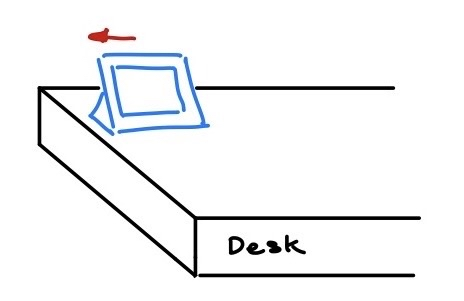
\includegraphics[width = \textwidth]{test_images/drop_1.jpg}
  \caption{First orientation}
  \end{subfigure}
  \begin{subfigure}[t]{0.5\textwidth}
  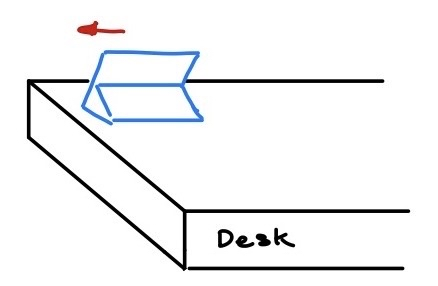
\includegraphics[width = \textwidth]{test_images/drop_2.jpg}
  \caption{Second orientation}
  \end{subfigure}
  \begin{subfigure}[t]{0.5\textwidth}
  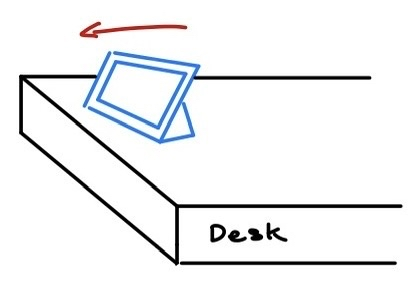
\includegraphics[width = \textwidth]{test_images/drop_3.jpg}
  \caption{Third orientation}
  \end{subfigure}
  \begin{subfigure}[t]{0.5\textwidth}
  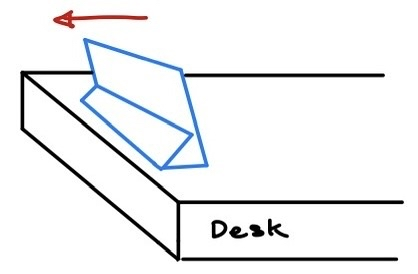
\includegraphics[width = \textwidth]{test_images/drop_4.jpg}
  \caption{Fourth orientation}
  \end{subfigure}
  \caption{Different drop orientations}
  \label{fig:orientations}
  \end{figure}

\item
  The device will be dropped once more, this time by having the tester
  hold the device facing themselves 100 centimeters above the ground and
  letting go of the device as shown in Fig.
  \ref{fig:drop}. Once again, images should be
  taken of the device and a functionality test must be performed after
  the drop.

  \begin{figure}
  \centering
  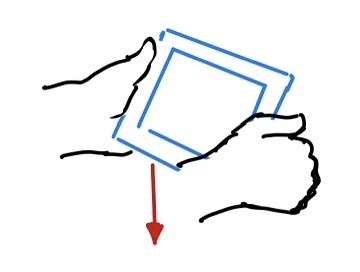
\includegraphics[width=0.5\textwidth]{test_images/drop_5.jpg}
  \caption{Final drop orientation}
  \label{fig:drop}
  \end{figure}
\end{enumerate}

Expectation: No cracking on the LCD screen and device remains fully
functional after all five drops. Minor defects on the plastic housing
are expected, but damage should be minimal without large cracks in the
plastic.

\pagebreak
\input{build/test_factoryReset_md}
\pagebreak
\input{build/test_lcd_md}
\pagebreak
\input{build/test_soundhaptics_md}
\pagebreak
\input{build/test_portDurability_md}
\pagebreak
\input{build/test_softwareUpdate_md}
\pagebreak
\input{build/test_tensile_md}
\pagebreak
\input{build/test_thermal_md}
\pagebreak
\input{build/test_thermalShock_md}
\pagebreak
\input{build/test_emi_md}
\pagebreak
\input{build/test_UV_md}
\pagebreak


\section{Review}
% Reflect on what went well and what you might do differently if you were to do it again
\input{akanksha_review_md}
\input{isabella_review_md}
\input{lennan_review_md}
\input{mason_review_md}
\input{sulaiman_review_md}

\end{document}
